\documentclass{simple}

\title[Despre manager]{De ce e greu să fii manager (bun)}
\institute{Excursie, Poiana Țapului}
\author[Răzvan Deaconescu]{Răzvan Deaconescu \\
razvan.deaconescu@upb.ro / razvand@unikraft.org}
\date{8 martie 2024}

\begin{document}

\frame{\titlepage}

\begin{frame}{Întâi de toate \ldots}
  \begin{figure}
    \centering
    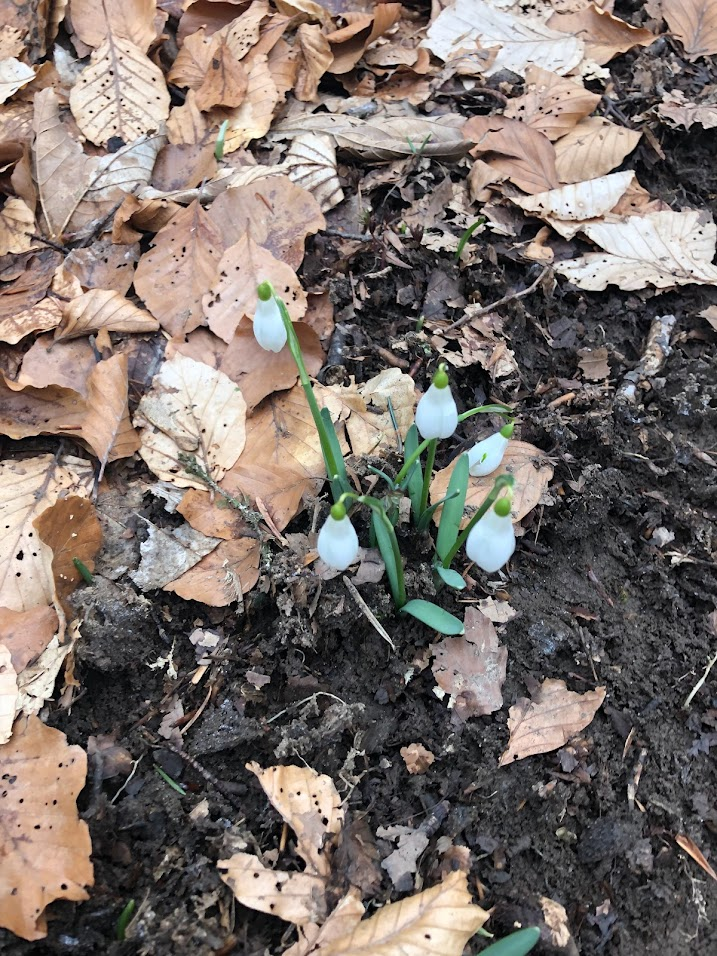
\includegraphics[width=0.4\textwidth]{img/snowdrop.jpg}
  \end{figure}
  \begin{center}
    La mulți ani, Adina, Alina, Andra, Andreea, Andreea, Andreia, Camelia, Crina, Delia, Ella, Emma, Giorgiana, Silvana!
  \end{center}
\end{frame}

\begin{frame}{}
  \begin{center}
    Cine este / Cine se consideră un manager?
  \end{center}
\end{frame}

\begin{frame}{Ce este un manager? Ce face un manager?}
  \begin{center}
    \pause
    gestionează lucrurile, are grijă de chestii \\
    \vspace{1cm}
    \pause
    se asigură că lucrurile se întâmplă
  \end{center}
\end{frame}

\begin{frame}{}
  \begin{figure}
    \centering
    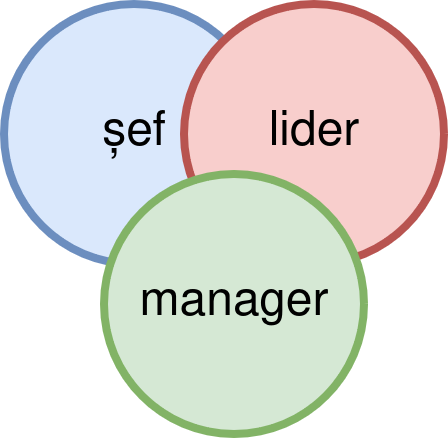
\includegraphics[width=0.7\textwidth]{img/sef-lider-manager.drawio.png}
  \end{figure}
\end{frame}

\begin{frame}{Manager de proiect vs. manager de echipă}
  \begin{center}
    \pause
    aceleași obiective: să se întâmple lucrurile, să existe rezultate \\
    \vspace{1cm}
    \pause
    focus diferit: proiect (metrici, documente, produse) vs echipă (stare de bine, unitate, ,,orchestră'')
  \end{center}
\end{frame}

\begin{frame}{De ce este nevoie de manageri?}
  \begin{center}
    \pause
    the world ain't saving itself \\
    \vspace{1cm}
    \pause
    stadiul natural este ,,entropic'' (haotic, dezorganizat, dezlânat)
  \end{center}
\end{frame}

\begin{frame}{}
  \begin{center}
    Cum stabilești ,,cantitatea de management''?
  \end{center}
\end{frame}

\begin{frame}{Ce face un manager? Ce face un dezvoltator?}
  \begin{center}
    \pause
    gestionează vs creează \\
    \vspace{1cm}
    \pause
    preocupat de ,,ansamblu'' vs preocupat de ,,specific'' \\
    \vspace{1cm}
    \pause
    responsabilități de rezultat vs. responsabilități tehnice \\
    \vspace{1cm}
    \pause
    lucrează cu oamenii vs. lucrează cu tehnologia
  \end{center}
\end{frame}

\begin{frame}{Cum ajungi manager (rol de manager)?}
  \begin{center}
    \pause
    vrei tu \\
    \vspace{1cm}
    \pause
    trebuie să fie cineva \\
    \vspace{1cm}
    \pause
    organic \\
    \vspace{1cm}
    \pause
    nu ai de ales
  \end{center}
\end{frame}

\begin{frame}{}
  \begin{center}
    Cum se manifestă un manager prost? Forme de management prost?
  \end{center}
\end{frame}

\begin{frame}{}
  \begin{center}
    Ce este un manager bun? Ce atribute / calități are?
  \end{center}
\end{frame}

\begin{frame}{De ce e greu să fii manager?}
  \begin{center}
    \pause
    personal (sine) \\
    \vspace{1cm}
    \pause
    inter-personal \\
    \vspace{1cm}
    \pause
    tehnic \\
    \vspace{1cm}
    \pause
    politic-organizațional
  \end{center}
\end{frame}

\begin{frame}{Personal}
  \begin{itemize}
    \pause
    \item doing it for the wrong reasons: bani, influență, career step, nu a vrut altcineva
    \pause
    \item De ce ai ajuns manager? Ce te face potrivit?
    \pause
    \item lipsă de plăcere autentică de a lucra cu oameni: ascultare, empatie, aliniere, sprijin emoțional, sprijin profesional, chit chat
    \pause
    \item sindromul impostorului, lipsă de deschidere, lipsă de feedback
  \end{itemize}
\end{frame}

\begin{frame}{Inter-personal}
  \begin{itemize}
    \pause
    \item orgoliu, eu sunt șef, general fără armată
    \pause
    \item control freakness, rigiditate, ,,eu știu mai bine''
  \end{itemize}
\end{frame}

\begin{frame}{Tehnic}
  \begin{itemize}
    \pause
    \item atenuare capacități tehnice, nu mai creezi, nu mai produci, nu mai construiești; facilitezi, coordonezi, organizezi
    \pause
    \item impact neagativ asupra celorlalți (,,oricum nu le mai are''), și asupra ta (,,eu nu fac, alții fac''), reacții compensatorii
  \end{itemize}
\end{frame}

\begin{frame}{Politic-organizațional}
  \begin{itemize}
    \pause
    \item prins la mijloc între nivelurile ierarhice: cerințe / nevoi de sus, posibilități de jos
    \pause
    \item presiune de a realiza obiective, stres
    \pause
    \item lipsa unei culturi de management bun; prioritizarea propriei persoane
    \pause
    \item risc de politicianism, carierism, gargară inutilă, să fie bine ca să nu fie rău
  \end{itemize}
\end{frame}

\begin{frame}{Cum să fii un manager (mai) bun?}
  \begin{center}
    Nu există rețete. Doar recomandări și bune practici.
  \end{center}
\end{frame}

\begin{frame}{Cum să fii un manager (mai) bun? (2)}
  \begin{center}
    \pause
    personal: micro-evaluations, instrospection \\
    \vspace{1cm}
    \pause
    inter-personal: true one-on-ones: Cum te simți? Ce îți direști? What can i do for you? \\
    \pause
    inter-personal: humbleness and openness \\
    \vspace{1cm}
    \pause
    tehnic: side hustle tehnic (nu hobbyuri ne-tehnice) \\
    \vspace{1cm}
    \pause
    politic-organizațional: coaie, creier și inimă: fermitate, diplomație și înțelegere
  \end{center}
\end{frame}

\begin{frame}{La final}
  \begin{center}
    Oricine este manager în anumite forme. \\
    \vspace{1cm}
    Cu cât suntem manageri mai buni în formele ,,organice'' cu atât putem fi manageri mai buni în formele organizate.
  \end{center}
\end{frame}

\end{document}
